%!TEX root = ../main.tex

\chapter{Costruzione di una rete e apprendimento}
\label{cha:euristiche_per_migliorare_l'apprendimento}

Quando si intende utilizzare una rete neurale per risolvere un particolare problema, ci sono diverse questioni da affrontare.
\begin{itemize}
	\item Da quanti strati dev'essere composta la rete?
	\item Quante unità sono necessarie per ogni strato?
\end{itemize}
Per rispondere a queste domande si introduce il concetto di \textbf{generalizzazione}.

\section{Generalizzazione}
\label{sec:generalizzazione}

\begin{mydef}[Generalizzazione]
	Con \defterm{generalizzazione} si intende la capacità di una rete di fornire risposte corrette ad esempi non incontrati durante la fase di addestramento (esempi di test).
\end{mydef}
\noindent Si assume che l'insieme di esempi di test (\emph{test set}) sia tratto dalla stessa popolazione usata per generare il training set.

Il problema di apprendimento può essere visto come un problema di \emph{approssimazione di una curva}: la rete è considerata semplicemente come una mappa input/output non lineare, dunque una buona generalizzazione è vista come una buona interpolazione dei dati di input.

Una rete progettata per generalizzare bene produce mappature input/output corrette anche se l'input è lievemente differente dagli esempi usati in fase di training: se però la rete viene addestrata con troppi esempi, si rischia di memorizzare il training set, ovvero la rete apprende il \textbf{rumore} presente nel training set. Questo fenomeno è detto \textbf{overfitting}: una rete \emph{sovra-addestrata} è troppo rigida e pertanto perde la capacità di generalizzazione.

In generale una rete troppo piccola impara poco, mentre una rete troppo grande impara molto, ma non generalizza abbastanza. In entrambi i casi si rischia di non riuscire a risolvere il problema: è necessario trovare un \emph{giusto compromesso}. 

\begin{figure}[h!]
	\centering
	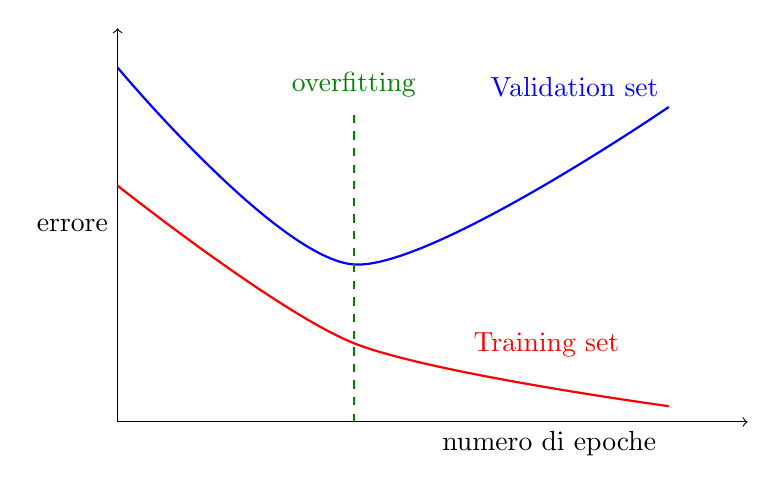
\begin{tikzpicture}
		\draw[->] (0,0) -- node[left] {errore} (0,5);
		\draw[->,below right] (0,0) -- node {numero di epoche} (8,0);

		\draw[thick, color=blue] plot [smooth, tension=0.5] coordinates{(0, 4.5) (3, 2) (7, 4)} node[above left] {Validation set};
		\draw[thick, color=red] plot [smooth, tension=0.5] coordinates{(0, 3) (3, 1) (7, 0.2)} node[above left=0.5cm] {Training set};
        
		\draw[thick, color=green!50!black, dashed] (3, 0) -- (3, 4) node[above] {overfitting};
        
	\end{tikzpicture}
	\caption[Andamento dell'errore e overfitting]{La curva rossa mostra l'andamento dell'errore nel classificare i dati di training, mentre la curva blu mostra l'errore nel classificare i dati di test o validazione. Se l'errore di validazione aumenta mentre l'errore sui dati di training diminuisce, ciò indica che siamo in presenza di un possibile caso di overfitting.}
\end{figure}

\begin{figure}[h!]
	\centering
	\includegraphics[width=10cm]{images/overfit2}
	\caption[Interpolazione e overfitting]{(a) dati del training set, (b) sotto approssimazione, (c) una buona stima sui dati, (d) overfitting: la curva di apprendimento è perfettamente disposta sul training set.}
\end{figure}

La capacità di generalizzazione è influenzata da \textbf{tre fattori} principali: le dimensioni del training set, l'architettura della rete neurale e la complessità del problema.

Dal momento che non si ha alcun controllo sulla complessità del problema, è possibile affrontare il problema della generalizzazione sotto due punti di vista differenti:
\begin{enumerate}
	\item l'architettura della rete è prefissata e lo scopo è determinare una dimensione del training set ottimale per una buona generalizzazione;
	\item la dimensione del training set è prefissata e lo scopo è di determinare la migliore architettura di rete per una buona generalizzazione.
\end{enumerate}

\section{Cross-validation}
\label{sec:cross_validation}

La \textbf{cross-validation} è una tecnica utilizzata per selezionare, tra un insieme di modelli utilizzabili per risolvere un problema, il modello migliore secondo certi criteri.

Durante un \textbf{round} di cross-validation si partiziona l'insieme di addestramento in due sottoinsiemi complementari:
\begin{itemize}
	\item \textbf{estimation subset}, usato per l'addestramento del modello;
	\item \textbf{validation subset}, usato per la validazione del modello.
\end{itemize}
La procedura viene iterata per diversi partizionamenti, al fine di ridurre la varianza dei risultati, e si calcola la media delle performance ottenute durante i diversi round.

Si distinguono solitamente due tipi di cross-validation:
\begin{itemize}
	\item \textbf{cross-validation esaustiva}, quando si considerano tutti i modi possibili per il partizionamento del training set (\textbf{leave-p-out} cross-validation);
	\item \textbf{cross-validation non esaustiva}, quando non si considerano tutti i possibili partizionamenti (\textbf{k-fold} cross-validation).
\end{itemize}
La tipologia di cross-validation più utilizzata è la $k$-fold cross-validation. In questo tipo di validazione, il training set è suddiviso in $k$ sottoinsiemi e si itera $k$ volte la seguente procedura: addestramento della rete su $k - 1$ sottoinsiemi e validazione sul rimanente. Ad ogni round si utilizza un diverso sottoinsieme come validation set.

Una volta selezionato il modello da utilizzare si ricorre al test set per verificare la capacità di generalizzazione della rete.

\begin{figure}[h!]
	\centering
	\begin{tikzpicture}[font=\scriptsize]
		\pie[pos={8,0},rotate=90, radius=1.2, color={black!40, black!20}]{75/ E, 25/ V}
		\pie[pos={12,0}, rotate=0, radius=1.2, color={black!40, black!20}]{75/ E, 25/ V}
		\pie[pos={8,-4}, rotate=270, radius=1.2, color={black!40, black!20}]{75/ E, 25/ V}
		\pie[pos={12,-4}, rotate=180, radius=1.2,  color={black!40, black!20}]{75/ E, 25/ V}
	\end{tikzpicture}
	\caption[Cross-validation]{Esempio di $4$-fold cross-validation: partizionamenti del training set in estimation subset E e validation subset V.}
\end{figure}

\section{Metodo di training early-stopping}
\label{sec:metodo_di_training_early_stopping}

Con l'obiettivo di una buona generalizzazione è molto difficile decidere quando è il momento di bloccare il training: c'è il rischio di overfitting dei dati se non si ferma l'addestramento al punto giusto.

Il processo di addestramento \textbf{early-stopping} è il seguente:
\begin{itemize}
	\item dopo un periodo di addestramento sull'estimation set, si calcola l'errore di validazione per ogni esempio del validation set;
	\item quando la fase di validazione è completa, si riprende la fase di addestramento per un altro periodo.
\end{itemize}
Se si osserva la sola curva dell'errore dell'estimation set (figura \ref{fig:overfit}), questo si riduce all'aumentare delle epoche ed è spontaneo pensare di proseguire l'addestramento anche oltre il punto di minimo della curva del validation set: in realtà ciò che la rete apprende dopo quel punto è il rumore contenuto nei dati del training set. L'euristica suggerisce quindi di fermare l'addestramento in corrispondenza del minimo della curva relativa al validation set.
\begin{figure}[h!]
	\centering
	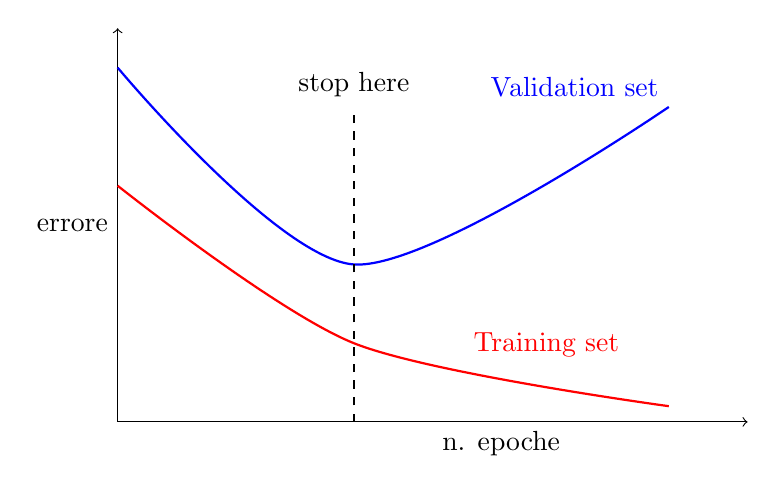
\begin{tikzpicture}
		\draw[->] (0,0) -- node[left] {errore} (0,5);
		\draw[->,below right] (0,0) -- node {n. epoche} (8,0);

		\draw[thick, color=blue] plot [smooth, tension=0.5] coordinates{(0, 4.5) (3, 2) (7, 4)} node[above left] {Validation set};
		\draw[thick, color=red] plot [smooth, tension=0.5] coordinates{(0, 3) (3, 1) (7, 0.2)} node[above left=0.5cm] {Training set};
        
		\draw[thick, dashed] (3, 0) -- (3, 4) node[above] {stop here};
        
	\end{tikzpicture}
	\caption{Andamento di errore e metodo di early stopping.}\label{fig:overfit}
\end{figure}

\section{Tecniche di pruning}
\label{sec:tecniche_di_pruning}

Le capacità funzionali e di generalizzazione di una rete sono fortemente influenzate dalla sua dimensione, ovvero il numero di neuroni nascosti. Con una rete troppo piccola si rischia di non riuscire a risolvere il problema, mentre con una troppo grande si rischia di apprendere il rumore deteriorando la capacità di generalizzare.

Per scegliere la dimensione corretta della rete si può procedere in due modi:
\begin{enumerate}
	\item \textbf{pruning}: si parte da una rete sovradimensionata per poi ridurla eliminando connessioni sinaptiche o neuroni interi;
	\item \textbf{growing}: si parte da una rete piccola per poi espanderla.
\end{enumerate}
Il primo approccio è tipicamente il più adottato: nonostante richieda maggior tempo computazionale, in quanto ci sono più unità da addestrare, è più veloce in termini di numero di epoche (convergenza più veloce) ed è del tutto indipendente dall'algoritmo di addestramento utilizzato.

Consideriamo per semplicità una rete con un singolo strato nascosto.
\begin{figure}[h!]
	\centering
	\begin{tikzpicture}[->,shorten >=2pt, shorten <= 2pt, auto, node distance=\layersep]
		\def\nodesep{-2cm}
		\def\layersep{4cm}
		% Draw the input layer nodes
		\foreach \name / \y in {1,...,3}
		\node[input neuron, pin=left:$x_\y$] (I-\name) at (0, \nodesep * \y) {};

		% Draw the hidden layer nodes
		\foreach \name / \y in {1,...,3}   
		\node[hidden neuron,  pin={[pin edge={->}]above:$y_\y$}] (H-\name) at (\layersep, \nodesep * \y + 1cm) {};
		
		\node[hidden neuron, color=black, text=white,  pin={[pin edge={->}]above:$y_h$}] (H-4) at (\layersep, \nodesep * 4 + 1cm) {$h$};
        
		% Draw the output layer nodes
		\foreach \name / \y in {1,...,3}   
		\node[output neuron, pin={[pin edge={->}]right:$O_\y$}] (O-\name) at (2*\layersep, \nodesep * \y) {};

		% Connect every node in the input layer with every node in the hidden layer.
		\foreach \source in {1,...,3}
		\foreach \dest in {1,...,3}
		\path (I-\source) edge (H-\dest);
                
		\foreach \source in {1,...,3}
		\path (I-\source) edge[dashed] (H-4);

		% Connect every node in the hidden layer with every node in the output layer.
		\foreach \source in {1,...,3}
		\foreach \dest in {1,...,3}
		\path (H-\source) edge (O-\dest);
                
		\foreach \source in {1,...,3}
		\path (H-4) edge[dashed] (O-\source);

		% Annotate the layers
		\node[annot,above of=H-1, node distance=2cm] (hl) {Hidden layer};
		\node[annot,left of=hl] {Input layer};
		\node[annot,right of=hl] {Output layer};
		\node[annot, below=2mm of H-4] (nh) {$n_h$};
		\node[annot, left of=nh] {$n_i$};
		\node[annot, right of=nh] {$n_o$};
	\end{tikzpicture}
	\caption{Rimozione del neurone $h$ in una rete neurale.}
\end{figure}

\noindent L'approccio del pruning consiste nel rimuovere un neurone $h$ e successivamente aggiustare i \textbf{pesi entranti} nelle unità servite da $h$ in modo tale da preservare il comportamento di input/output dell'intera rete. Questo è equivalente a risolvere il sistema
\begin{displaymath}
	\underbrace{\sum_{j = 1}^{n_h}  w_{ij} y^\mu_j}_\textrm{prima} = 
	\underbrace{\sum_{j = 1 \atop j \neq h} ^ {n_h} \left(w_{ij} + \delta_{ij} \right) y^\mu_j}_\textrm{dopo} \qquad \forall i = 1, \dots, n_o, \quad \forall \mu = 1, \dots, P
\end{displaymath}
dove $\delta_{ij}$ sono i fattori di aggiustamento da scoprire e $y_j^\mu$ è l'output dell'unità $j$ quando viene dato in input il pattern $\mu$.

L'equazione precedente può essere riscritta come
\begin{displaymath}
	\sum_{j = 1}^{n_h}  w_{ij} y^\mu_j = 
	\sum_{j = 1 \atop j \neq h} ^ {n_h} w_{ij} y^\mu_j + 
	\sum_{j = 1 \atop j \neq h} ^ {n_h} \delta_{ij} y^\mu_j
\end{displaymath}
da cui si ottiene
\begin{displaymath}
	\sum_{j = 1 \atop j \neq h} ^ {n_h} \delta_{ij} y^\mu_j =
	w_{ih} y^\mu_h
\end{displaymath}
che è un sistema lineare di equazioni con incognite $\{\delta_{ij}\}$.

È possibile scrivere il sistema in forma matriciale. Sia $N = (V, E, w)$ il grafo pesato che rappresenta la rete neurale da ridurre e siano $P_i$ e $R_i$ definiti come segue:
\begin{align*}
	P_i &= \{j : (i, j) \in E\} \\
	R_i &= \{j : (j, i) \in E\}
\end{align*}
Per ogni $i \in P_h$ definiamo la matrice $\mat{Y}_{i, h} = [\vec{y}_{j_1} \dots \vec{y}_{j_{r_i - 1}}]$, dove ogni colonna è l'output dell'unità $j_k \in R_i \setminus \{h\}$. Dobbiamo risolvere $|P_h|$ sistemi del tipo
\begin{displaymath}
	\mat{Y}_{i, h} \vec{\delta}_i = \underbrace{w_{ih} \vec{y}_h}_{\vec{z}_{i, h}}
\end{displaymath}
che possono essere combinati in un unico sistema
\begin{displaymath}
	\mat{Y}_h \vec{\delta} = \vec{z}_h
\end{displaymath}
dove
\begin{align*}
	\mat{Y}_h &= \diag(\mat{Y}_{i_1, h}, \dots, \mat{Y}_{i_{p_h}, h}) \\
	\vec{\delta} &= (\vec{\delta}_{i_1}^T \dots \vec{\delta}_{i_{p_h}}^T)^T \\
	\vec{z} &= (\vec{z}_{i_1}^T \dots \vec{z}_{i_{p_h}}^T)^T
\end{align*}
Dal momento che il sistema è sovradeterminato si può utilizzare il metodo dei minimi quadrati per approssimare una soluzione:
\begin{displaymath}
	\argmin_{\vec{\delta}} \|\mat{Y}_h \vec{\delta} - \vec{z}_h\|
\end{displaymath}
I fattori di aggiustamento così calcolati permettono di preservare il comportamento della rete avendo rimosso il neurone $h$.

Rimane ora da determinare come scegliere l'unità da rimuovere: idealmente, la scelta più appropriata sarebbe eliminare l'unità nascosta con il più piccolo \textbf{residuo finale} calcolato sul sistema corrispondente. Questo garantisce che la rimozione dell'unità avrà un impatto minimo sul comportamento della rete, tuttavia il calcolo del residuo minimo finale ha un costo computazionale elevato (a causa del numero di sistemi da risolvere, uno per ogni neurone nascosto).

Nella pratica si cerca pertanto una soluzione subottimale: i metodi di riduzione dei residui per risolvere il problema dei minimi quadrati (come CGPCNE) partono da una soluzione iniziale $\vec{\delta}_0$ e producono una sequenza di punti $\{ \vec{\delta}(k) \}$ tale per cui i residui
\begin{displaymath}
	r_k = \|\mat{Y}_h \vec{\delta}(k) - \vec{z}_h\|
\end{displaymath}
si riducono, ovvero $r_k \geq r_{k + 1}$. Un'approssimazione accettabile alla soluzione ottimale è scegliere l'unità $h$ con il più piccolo \textbf{residuo iniziale}. Dal momento che $\vec{\delta}(0)$ è solitamente il vettore nullo si ha
\begin{displaymath}
	\vec{\delta}(0) = \vec{0} \implies r_0 = \| \vec{z}_h \|
\end{displaymath}
e quindi si deve scegliere l'unità con $\| \vec{z}_h \|$ minimo. Naturalmente questo criterio non garantisce la soluzione ottimale, in quanto non è detto che partendo dal residuo iniziale minimo si giunga al residuo finale minimo, tuttavia nella pratica si è dimostrato efficace e semplice da implementare.

Riassumendo, data una rete sovradimensionata, i passi fondamentali dell'algoritmo di pruning sono i seguenti:
\begin{algorithmic}[1]
	\State Trovare l'unità $h$ con $\| \vec{z}_h \|$ minimo.
	\State Risolvere il sistema corrispondente (aggiustare i pesi).
	\State Rimuovere l'unità $h$.
	\State Ritorna al punto 1 se $Performance(pruned) - Performance(original) < \epsilon$, altrimenti scarta l'ultima rete ridotta.
\end{algorithmic}
